\clearpage
  \section{Mobile Security Mechanisms}

    There are a variety of different operating systems on mobile devices, offering different kind of security mechanisms. This section will give a brief introduction to the most popular operation systems on mobile devices and the supported security mechanisms.
    

    \subsection{Windows phone}

    \subsection{Ios}

    Apple launched it first mobile phone in xxxx called ``iphone'' with the operating system called ``IOS''. This section will give a introduction to its security mechanisms that are in use on the newest versions of ``Ios'' that are in use today. The newest ios devices are able to use two different locking mechanisms called Passcode and Touch ID. The passcode is a four-digit numeric pin. The user are authenticated by entering their secret passcode, e.g. the four-digit numeric code. The Touch ID is a physical unit build into the home button on the phone. Whenever the user touch the button while the phone is locked, the unit will record the users fingerprint used to authenticate the user. The touch ID is known as a biometric authentication scheme, e.g. ``something you are''.

    \begin{figure}[H]
      \centering
      \subfigure{
        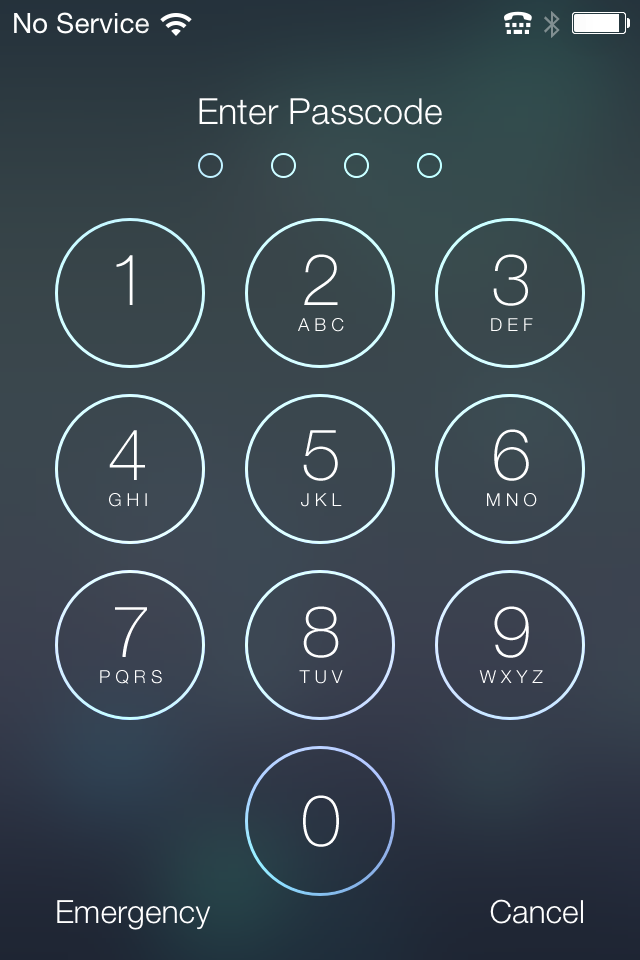
\includegraphics[scale=0.20]{pics/iosPasscode.png}
      }
      \subfigure{
        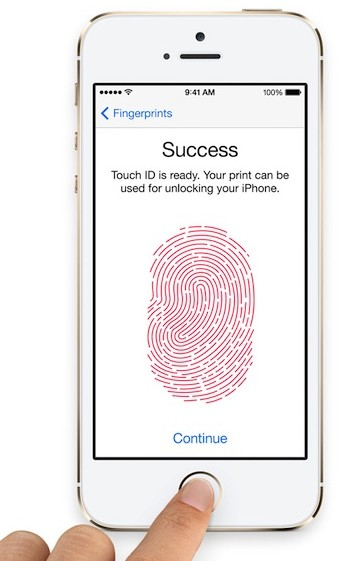
\includegraphics[scale=0.35]{pics/iosTouchID2.jpg}
      }
      \caption{1) Passcode 2) Touch ID }
    \end{figure}

  \clearpage
    \subsection{Android OS}

      \begin{itemize}
        \item None
        \item Swipe
        \item Face Recognition
        \item PIN code
        \item Pattern
        \item Password
      \end{itemize}

    
      \subsection*{Android Unlock Pattern}

      \begin{wrapfigure}{r}{0.35\textwidth}
      \vspace{-20pt}
      \begin{center}
        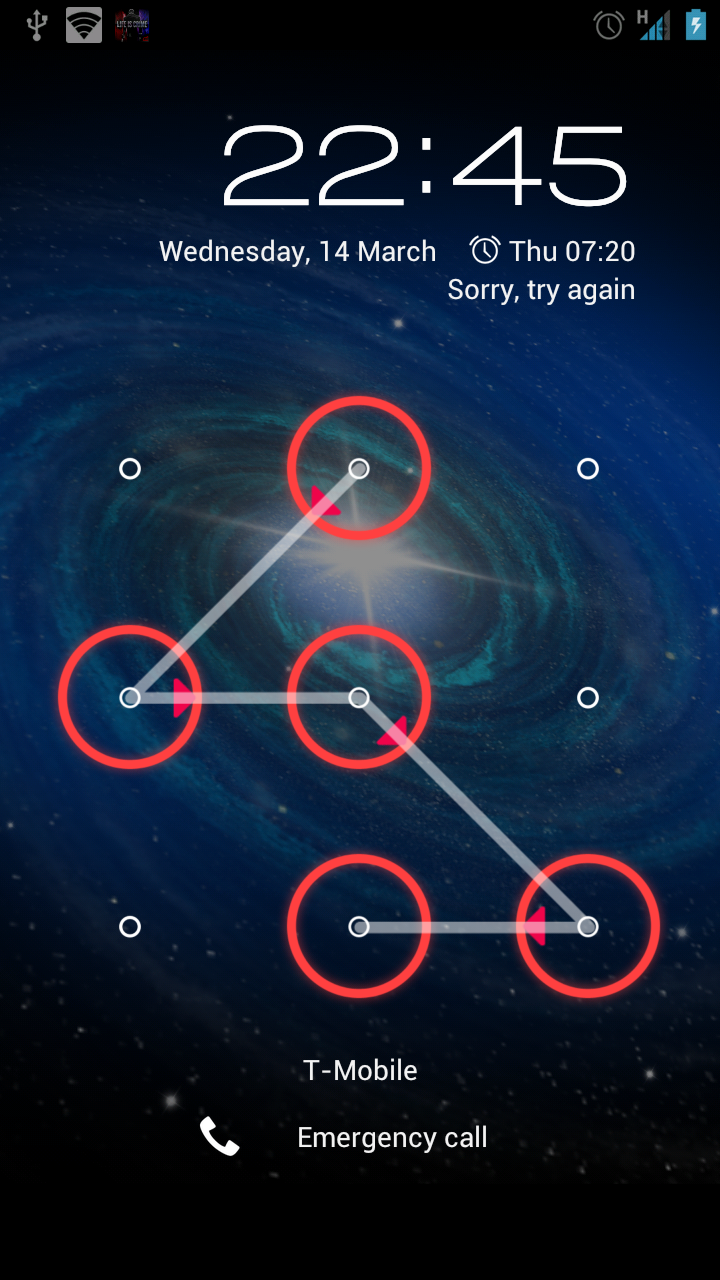
\includegraphics[scale=0.2]{pics/patternLock.png}
      \end{center}
      \vspace{-5pt}
      \caption{Usability vs. Security}
      \vspace{-10pt}
    \end{wrapfigure}

      The Android Unlock Patterns are a simplified version of the Pass-Go scheme that was proposed by Tao and Adams in 2008, and can be seen as a successor of the Draw-a-Secret (DAS) scheme. Both Pass-Go, Draw-a-Secret, and Android Unlock Patterns is categorized as recall-based authentication schemes.

      The Android password patterns are a simplified version of the Pass-Go scheme using a 3x3 grid, instead of a 9x9 as the Pass-Go scheme originally was designed. The Pass-Go scheme was inspired from the Chinese board game ``Go''.

      The settings on Android phones provides a default setting for using the Unlock pattern. 
      The rules are simple: 
          \begin{enumerate}
              \item At least four points must be chosen,
              \item You cannot visit the same node twice.
              \item Only straight lines are allowed, and
              \item One cannot jump over point not visited before
          \end{enumerate}